\UseRawInputEncoding
\documentclass[12pt, letterpaper] {article}
\usepackage{natbib}
\usepackage{amsmath, amsthm, amssymb, mathrsfs,array}
\usepackage{graphicx,float,wrapfig,subfigure,color,pdfpages,fixltx2e,url}



\pagestyle{plain}
\setlength{\parskip} {11pt}
\setlength{\parindent} {2em}
\setlength{\textwidth}{6.5in}
\setlength{\oddsidemargin} {0in}
\setlength{\textheight} {8.5in}
\setlength{\topmargin} {-0.5in}
\parskip 7.2pt

\newcommand{\nnub}{\nonumber}
\newtheorem{theorem}{Theorem}
\newtheorem{lemma}{Lemma}
\newtheorem{transform}{Transformation}
\newtheorem{corollary}{Corollary}
\newtheorem{property}{Property}
%\newtheorem{proposition}{Proposition}[section]
\newtheorem{proposition}{Proposition}
\newtheorem{definition}{Definition}
%\newtheorem{algorithm}{Algorithm}

\usepackage{algorithm}
\usepackage{algorithmic}

\newtheorem{assumption}{Assumption}
\newtheorem{observation}{Observation}

\renewcommand{\baselinestretch}{1.5}

\newcommand{\vocab}[1]{\textcolor{red}{#1}}

\begin{document}
	\title{NUS Business School Honors Dissertation}
	\author{Peng Seng Ang \\[0.5cm] {Advised by: Professor He Long}}
	\date{AY 2019/2020 Semester 2}
	\maketitle
\begin{abstract}
\noindent Many real industry problems involves spatio-temporal demand prediction, which requires predicting demand at a certain time across different locations. Most of the demand data are not continuous variables but instead count variables, like number of orders and number of transactions. Previous research have mainly explored neural network methods for spatio-temporal problems. In this paper, we focus on how we can apply classical time series model, using Vector Autoregressive models to exploit spatial correlations as well as introduce a 3-step approach to improve forecast accuracy. 

\end{abstract}
\newpage
\section{Introduction}

The motivation for this paper comes from \cite{Sheng2018}, where their focus is to optimise assignments of orders to drivers in order to minimize the total delay of all drivers. The dataset used in both \cite{Sheng2018} and this paper are from a food service provider in China that allows customer to place orders before a cutoff time in the day (e.g 10.00am) and the customer can expect to recieve their orders by a deadline (e.g anytime from 10.30am to 11.45am). 

\noindent The problem is not only restricted to the abovementioned food provider. With the rise of e-commerce and the food ordering and delivery services, like GrabFood and FoodPanda, demand prediction and driver assignment problem would be an everyday concern for them too. 

\noindent In reality, demand is never deterministic and hence, having an accurate forecast of demand for the food service providers would help them more effectively and efficiently assign orders to drivers to improve the overall delivery time. As such, the focus of this paper would be to accurately model and forecast the demand at the different locations and time. Currently, most Autoregressive (AR) or Autoregressive Integrated Moving Average (ARIMA) models only consider temporal features when predicting demand. However, we believe including spatial features between the data points might improve forecast accuracy. In this paper, classical time series models, such as Generalized Linear Model (GLM), ARIMA, as well as Vector Autoregressive (VAR) models, that include both spatial and temporal features would be explored. We also introduce a 3-step approach that combined unsupervised learning and supervised learning methods to improve forecast accuracy. 

\newpage
\section{Literature Review}
\cite{Marina2016} describes and shows how they implemented a network autoregressive moving average model to model the number of cases of Mumps in UK counties. In their example, they also showed that they might achieve a better result by modelling the series separately as univariate time series, also suggested in \cite{Nunes2015} since the neighbouring counties does not provide a substantial amount of explanatory power.  Other related literature includes \cite{Xavier2005} where they propose a model building strategy for spatially sparse but temporally rich data. 

\noindent BigVAR and tscount are some libraries that would be used in this paper. \cite{Tobias2017} provides the mathematical background and implementation of Generalised Linear Models (GLM) for count time series as a library (tscount) in R while \cite{William2017} extensively descibes the background and implementation of the VAR models and BigVAR library for multi-variate time series.

\noindent There are also various research on different methods used to predict spatio-temporal demand. One example would be \cite{Abolfazl2017}, where they proposed using generalized spatio-temporal autoregressive model for predicting taxi demands across locations in New York City. While most existing research regarding spatio-temporal forecasting makes use of deep learning methods, this paper would be more focused on using classical statistical method instead as it is more interpretable than deep learning neural networks.

\section{Data}
The data source used was an operational dataset from a food delivery service provider from Shanghai that includes delivery information for a 2-month period from 10 August 2015 to 30 September 2015 (excluding Saturdays) in 2015. The provider only provides delivery service for 90 minutes during lunchtime and the dataset has split the data into 15-minute time periods, and as such, each day would only consists of demand data for 6 time periods. Hence, our dataset has 839 locations with demand count data, in integer, for 204 time periods in total. 

\noindent To include other exogenous variables, data from https://www.worldweatheronline.com/shanghai-weather-history/shanghai/cn.aspx was used to include weather and rainfall data as well as encoding of the weekadys for all the respective days. 

\subsection{Exploratory Analysis}
We would first do some exploratory analysis and check if there are any interesting relationships between the variables. 

\begin{figure}[H]
    \centering
    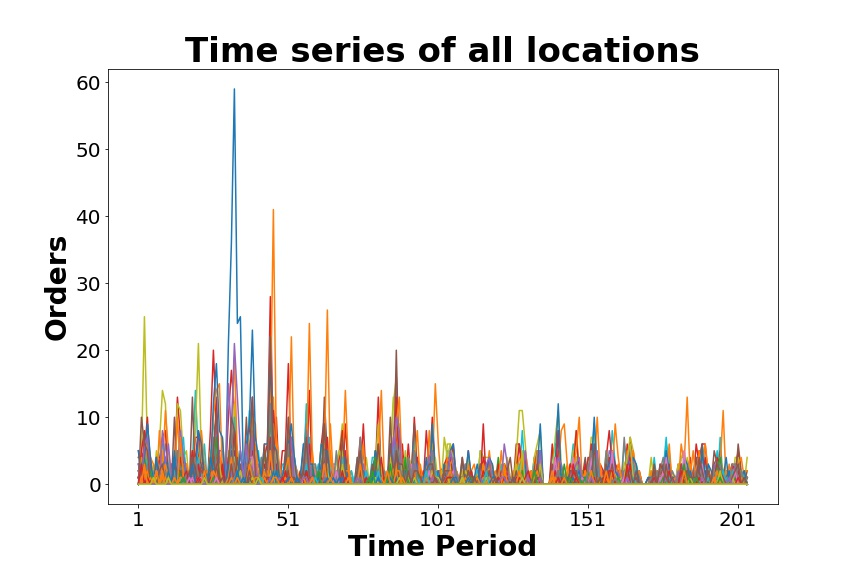
\includegraphics[width=0.95\textwidth, height=0.5\textheight]{Images/example_all_ts.jpg}
    \caption{Time series of all locations in the dataset. It can be observed that most locations have very low number of orders across the time period.}
    \label{fig:Time series of all locations in the dataset. It can be observed that most locations have very low number of orders across the time period.}
\end{figure}


\begin{figure}[H]
    \centering
    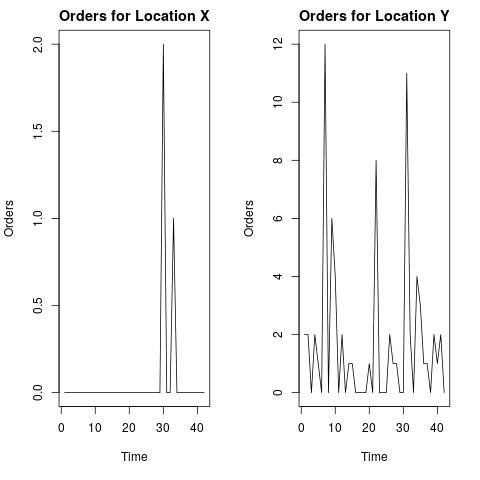
\includegraphics[width=\textwidth, height=0.35\textheight] {Images/example_ts.jpg}
    \caption{Most locations have very sparse time series (left) while some have relatively more dense time series (right)}
    \label{fig:Most locations have very sparse time series (left) while some have relatively more dense time series (right)}
\end{figure}


\begin{figure}[H]
    \centering
    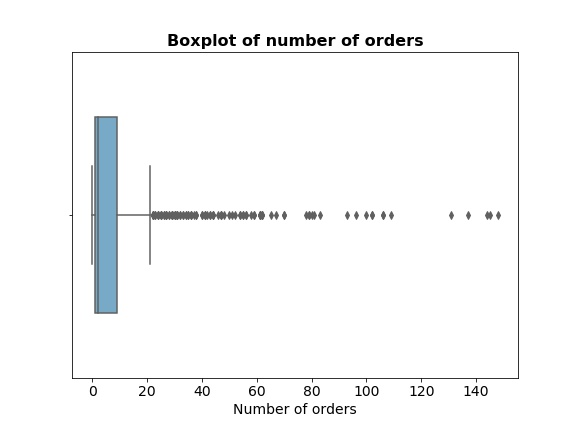
\includegraphics[width=\textwidth, height=0.35\textheight]{Images/boxplot_counts.jpg}
    \caption{Boxplot of counts. We can see that most of the locations have extremely low number of non-zero orders and further analysis showed that about 335 locations have just a maximum of one non-zero order throughout the 204 time periods.}
    \label{fig:Boxplot of counts. We can see that most of the locations have extremely low number of non-zero orders and further analysis showed that about 335 locations have just a maximum of one non-zero order throughout the 204 time periods. }
\end{figure}

\noindent Next, we observe how the demand changes across locations over time. 

\begin{figure}[H]
    \centering
    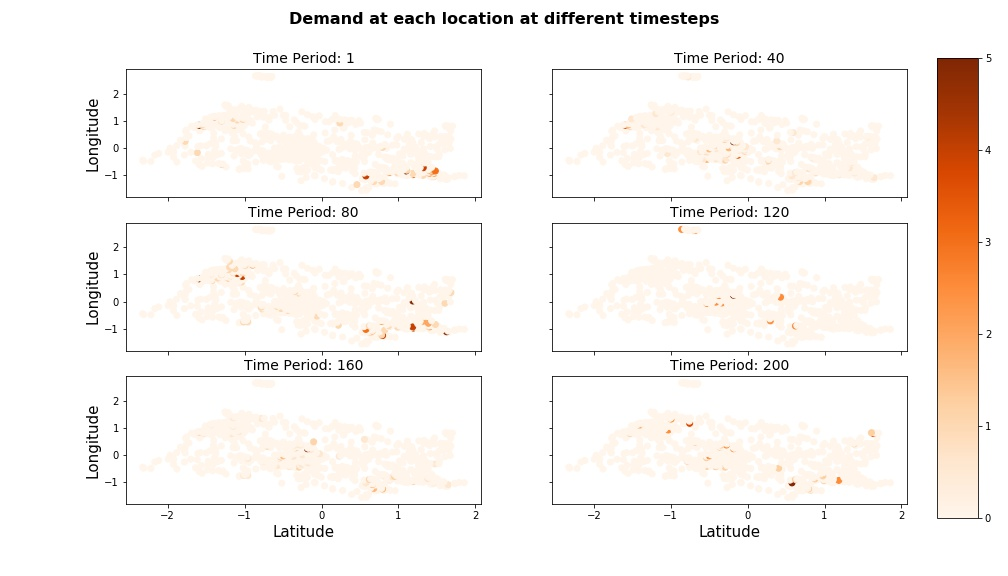
\includegraphics[width=0.95\textwidth, height=0.75\textheight]{Images/spatial_demand.jpg}
    \caption{Demand across locations over time}
    \label{fig:Demand across locations over time}
\end{figure}


\noindent We also performed some analysis on exogenous factors, such as the mean demand against temperature and against pressure. 

\begin{figure}[H]
    \centering
    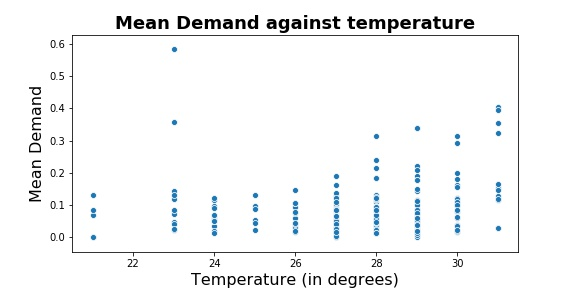
\includegraphics[width=0.95\textwidth, height=0.32\textheight]{Images/temp_mean_demand.jpg}
    \caption{Scatter plot of mean counts against temperature}
    \label{fig:Scatter plot of mean counts against temperature}
\end{figure}

\begin{figure}[H]
    \centering
    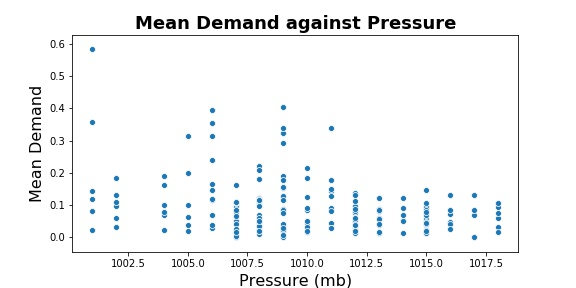
\includegraphics[width=0.95\textwidth, height=0.32\textheight]{Images/pressure_mean_demand.jpg}
    \caption{Scatter plot of mean counts against pressure}
    \label{fig:Scatter plot of mean counts against pressure}
\end{figure}

\noindent The scatter plot in Figure 4 visually display a slight positive relationship between temperature and mean demand across all locations whereas Figure 5 visually display a slight negative relationship between pressure and mean demand across all locations. We would explore usage and impact of the exogenous variables in predicting demand in the later portion of this paper. 



\subsection{Train-Test Split}
From Figure 1 in Section 3.1, the data is very sparse as there are many locations that have no demand counts for the majority of the time period. Hence, to get a better idea of how our models would work, only locations with at least 50 non-zero counts across the time period would be used initially, leaving us with 42 locations that meet this criteria. After the model is tested on the smaller dataset, we would then use the full dataset for location with at least one non-zero count to test and fit our model. 

\noindent To prevent overfitting of our model, the dataset was then split into training and test set by considering the first 33 days as the training set and the next 1 day as the test set. A period of 1 day was chosen as the test set duration because of the reasonable assumption that this model would only have to be run after the end of the day, hence only required to predict one-day ahead demand. 

\noindent Our training set would then have 198 demand data for each location and test set would have 6 demand data for each location. 

\section{Baseline Model}
In this section, we would build a simple baseline model, which is just fitting an ARIMA model on all the locations individually. Following which, we would try other different spatial temporal time series models and compare the results against the baseline model. 

\subsection{Metric Used}
The main metric that would be used for comparison would be Mean Squared Forecast Error (MSFE), which is calculated by:

\begin{center}
    %$\displaystyle MSFE=\frac{1}{(T_2 - T_1 - 1)}\sum_{t=T_1}^{T_2 - 1}\left \| \hat{y}_{t+1} - y_{t+1} \right \|_{2}^{2}$
    $\displaystyle MSFE=\frac{1}{n}\sum_{t=1}^{n}\left \| \hat{y}_{t} - y_{t} \right \|_{2}^{2}$
\end{center}
where \textit{n} is the number of data points, $\hat{y_t}$ is the predicted demand at time t and ${y_t}$ is the actual demand at time t.


\subsection{ARIMA models}
Autoregressive Integrated Moving Average (ARIMA) models are one of the most commonly used models for time series (\cite{Asha2016}). ARIMA models are made up of 3 processes, mainly the Autoregressive (AR) process, the Integrated (I) process and the Moving Average (MA) process (\cite{Jamal2018}). The AR process assumes that each observation can be expressed as a linear combination of its past values.  An AR(x) process would mean using x lagged values. The MA process assumes that each observation can be expressed as a linear combination of its current error term as well as its past error terms. The Integrated Process states that the time series can undergo differencing to ensure that the series is stationary. A MA(x) process would mean using x number of past observations. Hence, an ARIMA model is usually represented by ARIMA(p,d,q), where \textit{p} represents the number of autoregressive terms, \textit{d} represents the number of differences needed for stationarity, and \textit{q} represents the number of lagged forecast errors. 

\subsection{Baseline ARIMA Result}
As a baseline model, each of the locations was assessed individually and a suitable ARIMA model was built for each location. Auto-arima function from Python was used to implement this. The out-of-sample MSFE for this baseline model on the smaller dataset is \textbf{47.60} and MSFE for dataset of all locations is \textbf{72.48}. A sample forecast plot is shown below:

\begin{figure}[H]
    \centering
    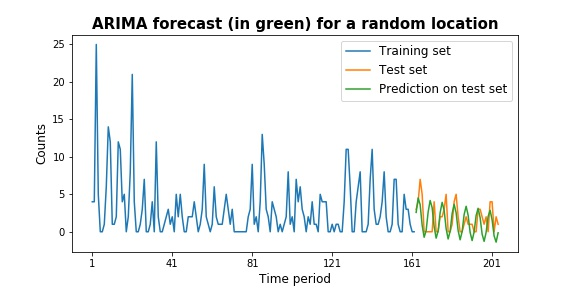
\includegraphics[width=\textwidth]{Images/forecast_example.jpg}
    \caption{ARIMA forecast on a random location}
    \label{fig:ARIMA forecast on a random location}
\end{figure}


\section{GLM Model}
The dataset that we are using follows a count time series, which means the observations are non-negative integers. A flexible and commonly used model for count time series is the Generalized Linear Model (GLM) \cite{Nelder1972}. GLM normally take the form of:

\begin{center}
    $\displaystyle g(\lambda_t)= \eta^T X_t$
\end{center}

\noindent where $g$ represents a link function, and $\lambda_t = E(Y_t | F_{t-1})$, where $F_{t-1}$ represents the historical values up to time t, which is the conditional mean of the time series . $\eta$ represents a parameter vector that corresponds to the covariates. $X_t$ represents the a vector of the values of the previous time steps in the time series.

%\noindent Using the R package from \cite{Tobias2017}, the GLM used would be an %extension of the above equation and can be expressed in the form of:

%\begin{center}
%    $\displaystyle g(\lambda_t)=\beta_0 + \sum_{k=1}^{p}\beta_k\tilde{g}(Y_{t-i_k}) + \sum_{\mathit{l}=1}^{q}\alpha_\mathit{l} g(\lambda_{t-j_\mathit{l}}) + \eta^T X_t$
%\end{center}

%\noindent where additionally, $\tilde{g}$ represents a transformation function. (remove this?)

\subsection{Model Implementation}
\noindent As mentioned in section 3.2, we would first assess our model on the smaller dataset before testing it on the full dataset. Using the R package tscount from \cite{Tobias2017}, we fit each of the locations individually by a GLM model. We used the past 6 lagged values as well as the indentity function as the link function. The out-of-sample MSFE for this baseline model on the smaller dataset is \textbf{38.16}, which is better than just using ARIMA on the same dataset.  

\noindent However, when it is implemented on the full dataset, the MSFE of the GLM increases to \textbf{82.42}, which is worse than just applying ARIMA on every location, which gives a MSFE of 72.48. 

\subsection{Model Diagnostics}
To validate and verify if our fitted model is adequate, model checking would be performed by performing the following residual analysis.		

\subsubsection{Residuals plots}

\begin{figure}[H]
    \centering
    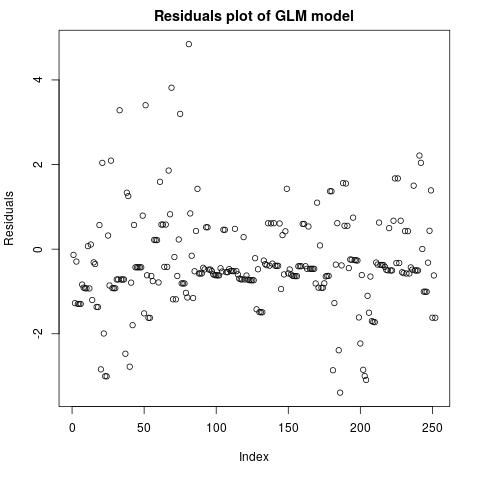
\includegraphics[width=\textwidth, height=0.7\textheight]{Images/Full_GLM_resids.jpg}
    \caption{Residuals for GLM Model}
    \label{fig:Residuals for GLM Model}
\end{figure}

\noindent Figure 7 diagnostic plots shows that while the residuals are roughly randomly scattered, the GLM model produces residuals that does not follow the normal distribution well. Although not ideal, this is expected as we assume that the distribution is poisson and not normal. 

\subsubsection{Residuals against Predicted values}

\begin{figure}[H]
    \centering
    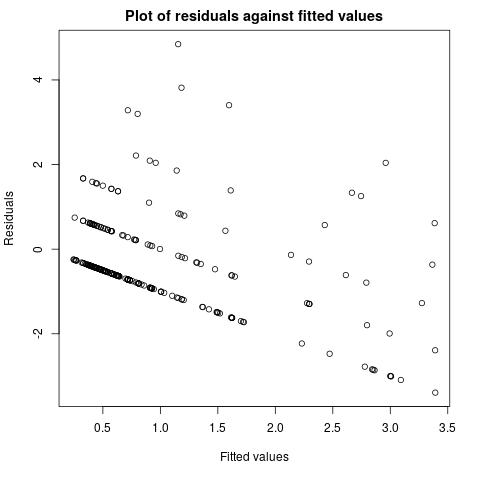
\includegraphics[width=0.85\textwidth, height=0.6\textheight]{Images/Full_GLM_resids_vs_fitted.jpg}
    \caption{Residuals against Predicted values for GLM Model}
    \label{fig:Residuals against Predicted values for GLM Model}
\end{figure}

\noindent The above plot of residuals against the predicted values suggests heteroscedasticity between residuals, or non-constant variance between the residuals as the predicted value increases, which is expected in a Poisson GLM, as mentioned in \cite{Dylan2017}. For a normal regression model, this would not be a desirable result but since we are assuming that our count data follows a Poisson distribution, the residuals are bound to display heteroscadasticity. 

\subsection{Model Limitation}

Similar to the baseline ARIMA model, it would be a relatively expensive and time-consuming process as every location has to be individually fitted to a GLM model. Also, each location model only uses its past values and does not take into account data from the other locations. The next section explores another type of model which would use data from other locations as predictors. 

\section{Vector Autoregressive (VAR) Model}

\subsection{Details of VAR Model}
Vector Autoregressive (VAR) models are the most commonly used model for multivariate time series, particularly in economics and financial time series as shown in \cite{Hilde2000}. VAR models are very similar to multivariate linear regression models and methods used to perform inferencing on linear regression models can also be applied to VAR models. VAR(p) represents a VAR model of order p if the time series can be written as: 

\begin{center}
    $\displaystyle y_t=v+\sum_{i=1}^{p} \phi_{i}y_{t-i}+\alpha_t$
\end{center}

\noindent where $p$ is the number of lagged endogenous variables used, $y_t$ is the value at time $t$, $v$ is a constant vector, $\phi_i$ are coefficient matrices for $i>0$ and $\alpha_t$ are independent and identically distributed random vectors. 

\subsection{Motivation}

As with many spatio-temporal demand prediction, spatial features could be an important feature if there exist spatial correlation. To check if there exist spatial correlation between the locations, a correlation heatmap would be plotted. For clear illustration purposes, instead of showing the matrix of correlation for all 839 locations, only the 42 locations with at least 50 non-zero counts would be shown. 

\begin{figure}[H]
    \centering
    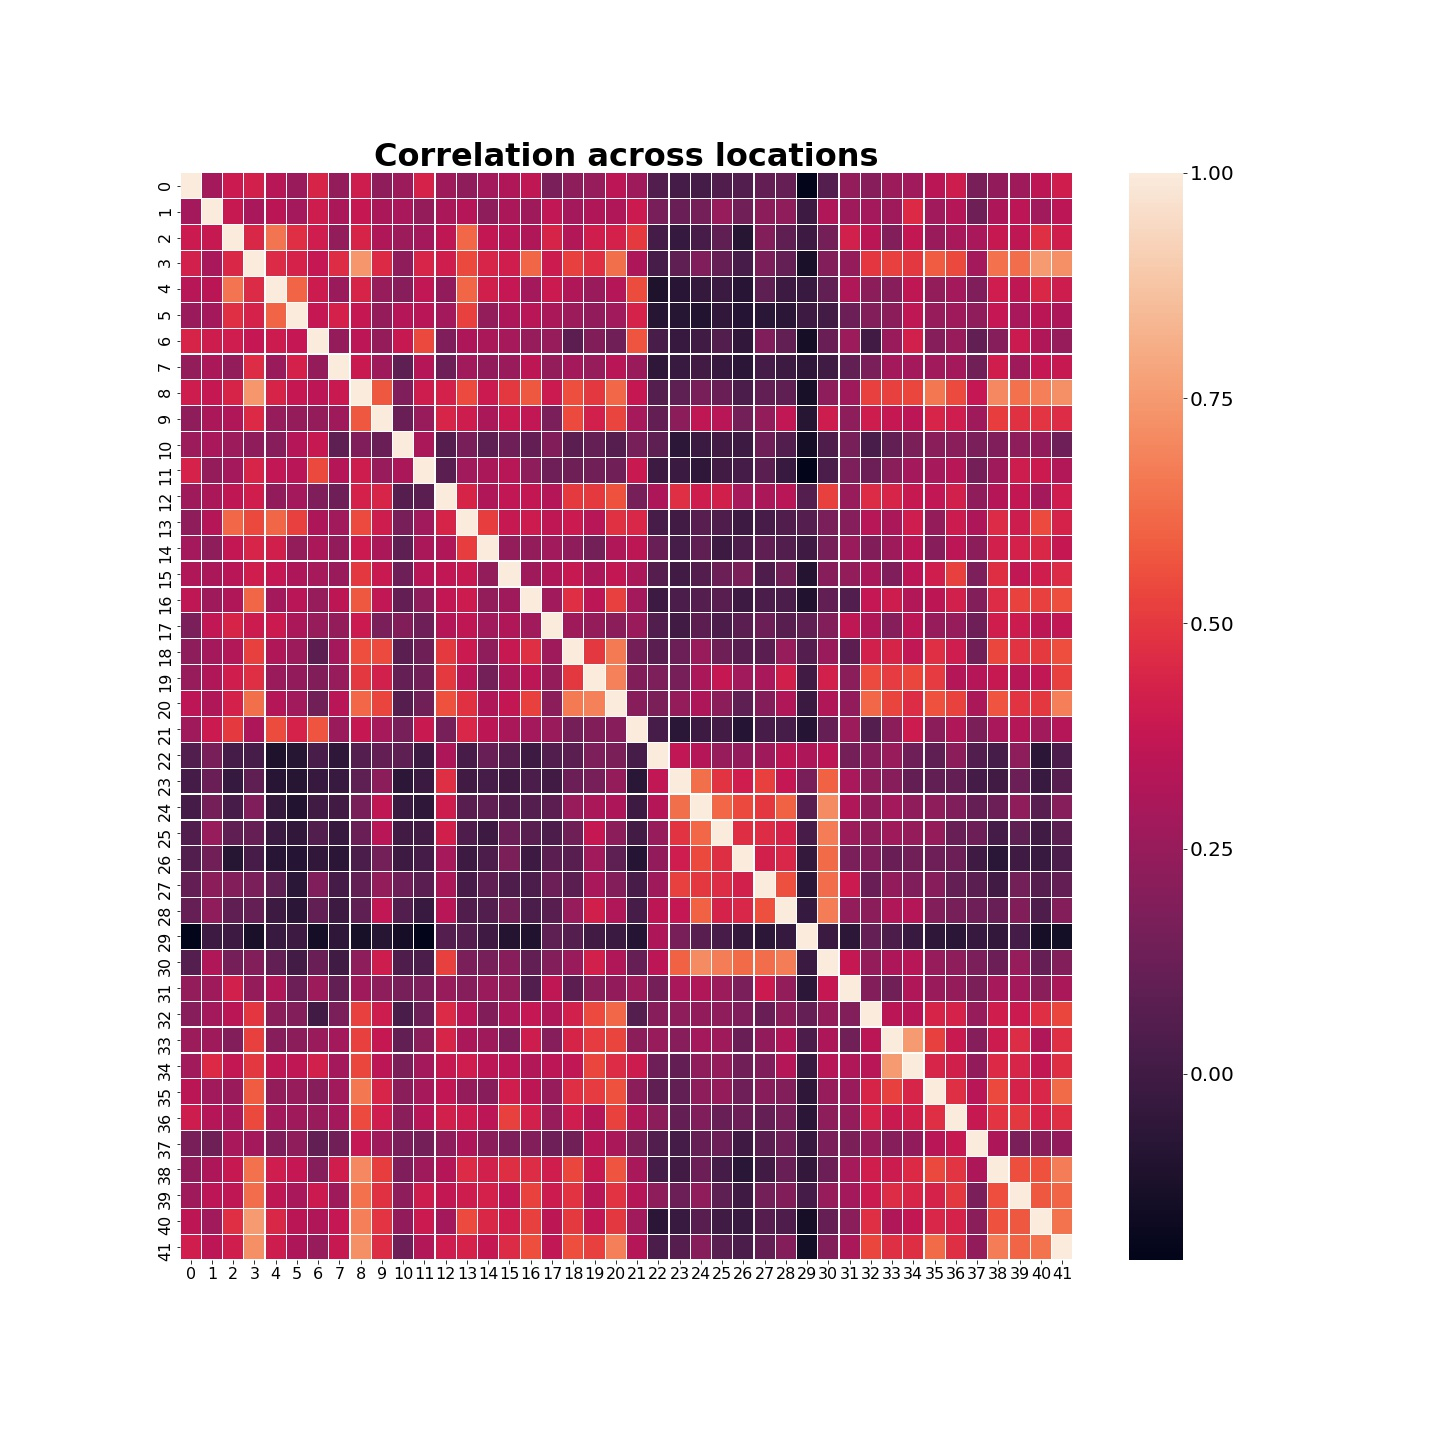
\includegraphics[width=\textwidth, height=0.75\textheight]{Images/heatmap.jpg}
    \caption{Spatial Correlation Heatmap on the locations with at least 50 non-zero counts. Axes represent the 42 locations}
    \label{fig:Spatial Correlation Heatmap. Axes represent locations}
\end{figure}

\noindent This thus provides the motivation to use the existence of spatial correlation and explore the usage of VAR model.

\subsection{Stationarity Condition}
For a univariate time series, it is important for the time series to be transformed into a stationary series and Augmented Dickey-Fuller (ADF) test can be used to perform unit root test for stationarity, as shown in \cite{Zhijie1998} and \cite{Rizwan2011}. For a multi-variate time series, if the series are unit-root non-stationary, regression models might show a statistially significant, but false, coefficients and results simply because the series are coincidentally increasing over time, hence applying the VAR model on non-stationary series could lead to spurious regression, also shown in \cite{Baumohl2009}.  


\subsection{Implementation of VAR Model for our dataset}

To test for stationarity, we would be performing the standard ADF test to test for stationarity. The result of the ADF test showed that time series of certain locations are not stationary. We then take the first difference of each series and after differencing, ADF test was performed on each series the time series of each location have been checked and are stationary. It is noted that while it is possible to perform differencing on every series, it might cause over-differencing, leading to inaccurate results, as mentioned in \cite{Ruey2014}.

\noindent Next, BigVAR Library in R was used to fit a VAR model with a maximum lag of 12, using time series of every location as predictors. The results for the VAR model is discussed in the later subsection. 

\subsubsection{Cointegration}
\cite{Box1977} shows that it is possible to linearly combine various unit-root nonstationary time series to form a stationary series. The term Cointegration, first mentioned in \cite{Granger1983}, states that although some or all the time series might be unit-root nonstationary individually, these time series can be said to be cointegrated if there exists a possible linear combination of them that would form a stationary series. Intuitively, 2 series are cointegrated if they move together and the distance between them remain stable over time. 

\subsubsection{Johansen Test for Cointegration}
While Cointegrated Augmented Dickey Fuller Test, commonly used for Pairs Trading, can be used, it is able to be applied on only 2 separate series. The next best approach is the cointegrating tests for VAR model, called the Johansen's Cointegration Test. However, one limitation is that it can only be used to check for cointegration between a maximum of 12 variables. For further elaboration on the Johansen's Cointegration Test, please refer to \cite{Johansen1991}. If there exists cointegration between variables, a Vector Error Correction Model can be formulated. 

\noindent However, since our dataset has 839 variables (locations), we are unable to apply the cointegration test or accurately calculate the significant values of more than 12 variables and hence unable to determine correctly the number of cointegration vectors needed. 

\subsection{VARX Model}
VAR models can also be extended to include exogenous variables. A VARX(p,s) (with exogenous variables) model can be expressed as:

\begin{center}
    $\displaystyle y_t=v+\sum_{i=1}^{p} \phi_{i}y_{t-i}+\sum_{j=1}^{s} \beta_{j}x_{t-j}+\alpha_t$
\end{center}

\noindent where $p$ is the number of lagged endogenous variables used, $s$ is the number of lagged exogenous variables used, $y_t$ is the value at time $t$, $v$ is a constant vector, $\phi_i$ are coefficient matrices for endogenous coefficient matrix for $i>0$, $\beta_i$ are coefficient matrices for exogenous coefficient matrix for $i>0$ and $\alpha_t$ are independent and identically distributed random vectors. 

\subsection{Implementation of VARX Model on our dataset}
\noindent Our dataset uses additional exogenous variables like temperature, wind, gust, cloud, humidity, precipitation, pressure as well as one-hot encoding of the day of the week. Our dataset now would have 839 endogenous variables/locations and 13 exogenous variables. Similarly, BigVAR library was used to fit a VARX model taking in the 839 locations' time series as endogenous variables and the 13 exogenous variables. 

\subsection{Model Checking}
To validate and verify if our fitted model is adequate, model checking would be performed by performing the following residual analysis:


\subsubsection{Whiteness of Residuals}
To ensure our fitted model is adequate, the resiudals should behave like a white noise series. 
The plots below shows the distribution of our residuals for the VAR model and the VARX model. 

\begin{figure}[H]
    \centering
    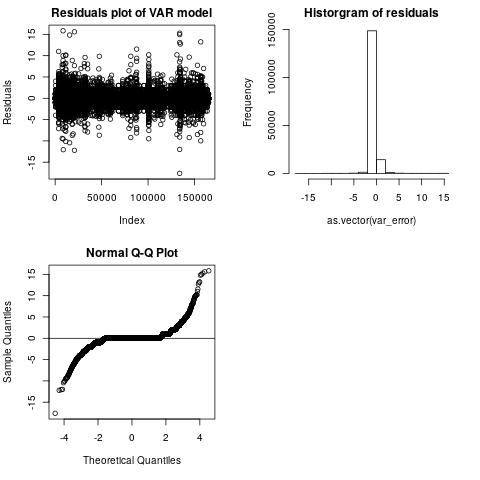
\includegraphics[width=0.8\textwidth, height=0.42\textheight]{Images/Full_VAR_diff_resids.jpg}
    \caption{Residuals for VAR Model}
    \label{fig:Residuals for VAR Model}
\end{figure}

\begin{figure}[H]
    \centering
    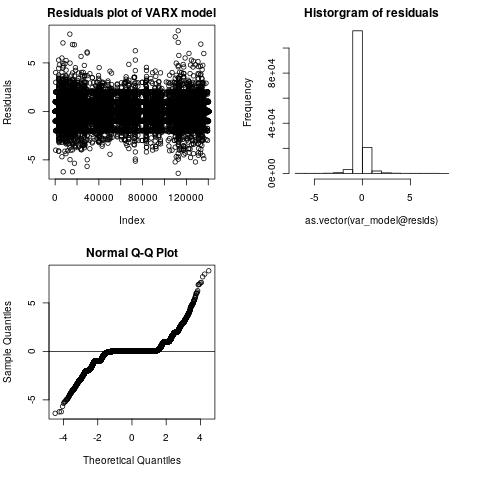
\includegraphics[width=0.8\textwidth, height=0.42\textheight]{Images/Full_VARX_diff_resids.jpg}
    \caption{Residuals for VARX Model}
    \label{fig:Residuals for VARX Model}
\end{figure}

From Figure 11 and 12, we can see that the residuals are mostly randomly scattered and they roughly follow a normal distribution, although it performs rather badly on the lower end and higher end of the outliers. 


\subsubsection{Residuals against Fitted Values}

\begin{figure}[H]
    \centering
    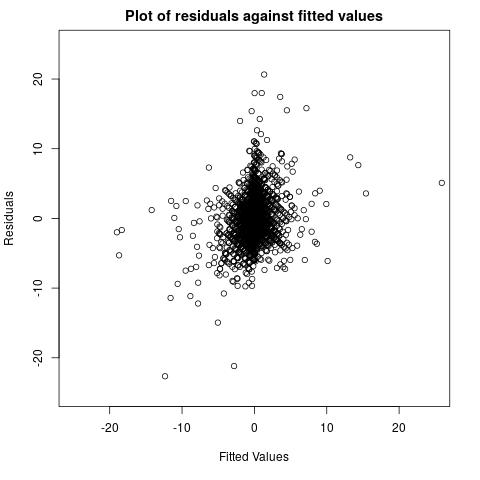
\includegraphics[width=0.6\textwidth, height=0.3\textheight]{Images/Full_VAR_diff_resids_vs_values.jpg}
    \caption{Residuals against Fitted Values for VAR Model}
    \label{fig:Residuals against Fitted Values for VAR Model}
\end{figure}

\begin{figure}[H]
    \centering
    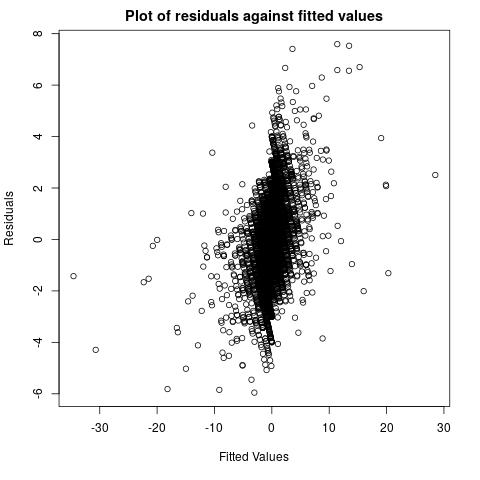
\includegraphics[width=0.6\textwidth, height=0.3\textheight]{Images/Full_VARX_diff_resids_vs_values.jpg}
    \caption{Residuals against Fitted Values for VARX Model}
    \label{fig:Residuals against Fitted Values for VARX Model}
\end{figure}

Figure 13 and 14 shows that heteroscadasticity occurs at the lower and higher ends of the predicted values, whereas in the middle range, the residuals tend to be roughly randomly scattered.

\subsection{Results}
BigVAR library in R was used to implement the VAR models. The MSFE for the VAR model is 76.72 and MSFE for VARX model is 75.63. Since the VARX includes exogenous variables and have a better result compared to the VAR model, it shows that the exogenous variables used do have a moderate amount of explanatory power. 

\section{3-step Approach}

Next, we would introduce an alternative 3-step approach, which is described here:

\noindent Step 1. Perform Clustering on the time series using one of the distance metric: 

	1.1 Euclidean distance between geo-location coordinates
	
	1.2 Correlation between time series 
	
	1.3 Dynamic Time Warping (DTW) distance between time series
	
	
	
\noindent Step 2. Aggregate the clusters and train a VAR model to predict the total demand for each cluster. 

\noindent Step 3. Re-allocate the total demand of each cluster to each location in the cluster while maintain a relative constant distribution as before.






%\begin{algorithm}
%\caption{3-Step Approach}
%\begin{algorithmic}
%\REQUIRE $n \geq 0 \vee x \neq 0$
%\ENSURE $y = x^n$
%\STATE 1. Cluster the time series.
%\IF{$n < 0$}
%\STATE $X \leftarrow 1 / x$
%\STATE $N \leftarrow -n$
%\ELSE
%\STATE $X \leftarrow x$
%\STATE $N \leftarrow n$
%\ENDIF
%\WHILE{$N \neq 0$}
%\IF{$N$ is even}
%\STATE $X \leftarrow X \times X$
%\STATE $N \leftarrow N / 2$
%\ELSE[$N$ is odd]
%\STATE $y \leftarrow y \times X$
%\STATE $N \leftarrow N - 1$
%\ENDIF
%\ENDWHILE
%\end{algorithmic}
%end{algorithm}

\noindent Similar methods can be found in \cite{Paul2015} and \cite{Chi2014}

\noindent 
\subsection{Clustering}

A simple K-means clustering was first done on the locations using their time series data in the training set. 3 different kind of distance metrics were used to perform K-means clustering. 

\noindent The first metric used would be to cluster based on their geo-locations while the second and third metric used would be to cluster them based on similarity between their historical time series. 

\subsubsection{Using longitude/latitude as the distance metric}

A reasonable assumption that could be made is that customers in the same neighbourhood would tend to have similar ordering behaviour due to similar residential status or similar working industry or culture. Hence, we would cluster the locations using their geo-location coordinates (longitude and latitude). K-means clustering is performed using the euclidean distance of the locations as the distance metric.   

\subsubsection{Using Correlation Coefficient as the distance metric}

We then also explored using correlation coefficient between the time series as the distance metric for K-means clustering. Correlation coefficient can be calculated by: 

\begin{center}
$r_{xy} = \frac{\sum_{i=1}^{n} (x_i - \overline{x})(y_i - \overline{y})}
{\sqrt{\sum_{i=1}^{n} (x_i - \overline{x})^2(y_i - \overline{y})^2}} $
\end{center}

\noindent where $r_{xy}$ represents the correlation coefficient between time series x and y, $x_i$ and $y_i$ represents points in time i for time series x and y respectively and $\overline{x}$ and $\overline{y}$ represents the mean value for time series x and y. Correlation measures the strength and direction of the tendency for any 2 time series to move together. 

\subsubsection{Using Dynamic Time Warping as the distance metric}

Finally, we explored using Dynamic Time Warping (DTW) Distance as the distance metric for K-means clustering. 

\noindent DTW is one of the commonly-used algorithm for measuring similarity between time series by providing a elastic non-linear alignment between 2 time series. It is known for being effective for time series that have different length or speed. DTW is calculated by first creating a distance matrix and then finding the optimal warping path as shown in the 2 algorithms here:

\begin{algorithm}[H]
\caption{Dynamic Time Warping (DTW) Algorithm to form distance matrix}
\begin{algorithmic}
%\REQUIRE $n \geq 0 \vee x \neq 0$
%\ENSURE $y = x^n$
\STATE 
\STATE 1. Initialise a 2-dimensional matrix M, where the indices of the rows and indices of the columns represent each point in time series x and time series y. 
\STATE 2. Populate the matrix from bottom-left to top-right with each element $c_{i,j}$ of the matrix representing the distance between $x_i$, the $i^{th}$ element of time series x and $y_j$, the $j_{th}$ element of time series y, which is calculated by:

\begin{center}
$c_{i,j} = (x_i - y_j) + min(c_{i-1,j}, c_{i,j-1}, c{i-1,j-1})$
\end{center}

\end{algorithmic}
\end{algorithm}

\begin{algorithm}[H]
\caption{Using DTW Matrix to find optimal warping path}
\begin{algorithmic}
\REQUIRE i*j distance matrix from DTW Algorithm
%\ENSURE $y = x^n$
\STATE Let i = rows(matrix) and j = columns(matrix)
\STATE Let path = []
\WHILE {(i != 1) and (j != 1)}
\IF{i==1}
\STATE $j = j-1$
\ELSIF{j==1}
\STATE $i = i-1$
\ELSE
\IF{matrix[i-1,j] == min(matrix(i − 1, j), matrix(i, j − 1), matrix(i − 1, j − 1))}
\STATE $i = i - 1$
\ELSIF{matrix[i,j-1] == min(matrix(i − 1, j), matrix(i, j − 1), matrix(i − 1, j − 1))}
\STATE $j = j - 1$
\ELSE
\STATE $i = i - 1, j = j - 1$
\ENDIF
path.add((i,j))
\ENDIF
\ENDWHILE
\RETURN path
\end{algorithmic}
\end{algorithm}


%\IF{$n < 0$}
%\STATE $X \leftarrow 1 / x$
%\STATE $N \leftarrow -n$
%\ELSE
%\STATE $X \leftarrow x$
%\STATE $N \leftarrow n$
%ENDIF
%WHILE{$N \neq 0$}
%\IF{$N$ is even}
%\STATE $X \leftarrow X \times X$
%\STATE $N \leftarrow N / 2$
%\ELSE[$N$ is odd]
%\STATE $y \leftarrow y \times X$
%\STATE $N \leftarrow N - 1$
%\ENDIF
%\ENDWHILE
%\end{algorithmic}
%\end{algorithm}
\newpage
\noindent We can also understand DTW visually by:

\begin{figure}[H]
    \centering
    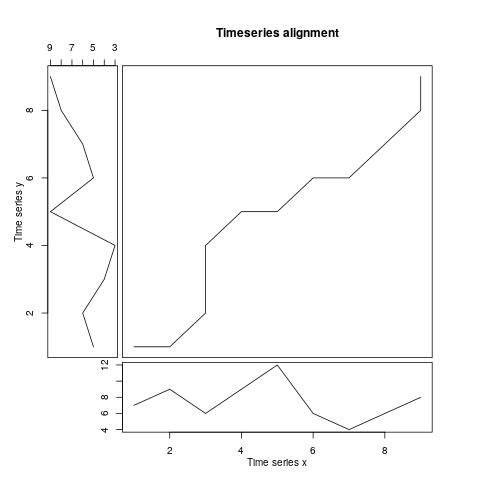
\includegraphics[width=0.8\textwidth, height=0.5\textheight]{Images/DTW_Plot.jpg}
    \caption{DTW Alignment Plot}
    \label{fig:DTW Alignment Plot}
\end{figure}

\noindent The plot in the middle shows the optimal warping path between the 2 time series. The distance is calculated by the euclidean distance between the points of the 2 time series that lie along the warping path as shown in:

\begin{center}
$DTW Distance = \sqrt{\sum_{(i,j)\in {Warping Path}}(x_i - y_j)^2}$
\end{center}

\noindent More details on the applications and optimisation of DTW can be found in \cite{Pavel2008}  
\newpage 

\subsection{Predicting total demand for each cluster}

\noindent We first aggregate the locations of each cluster together such that:

\begin{center}
$x\:\epsilon \: C(i)$
\end{center}

\begin{center}
$D_{C(i)} ={\sum_{l\epsilon C(i)}\sum_{j=1}^{n}x_{lj}}$ 
\end{center}

\noindent if location x belongs to Cluster i and where $D_{C(i)}$ represents the total demand (from training set) of the cluster C(i) and $x_{ij}$ represents the training set demand at location i at time j. 

\begin{figure}[H]
    \centering
    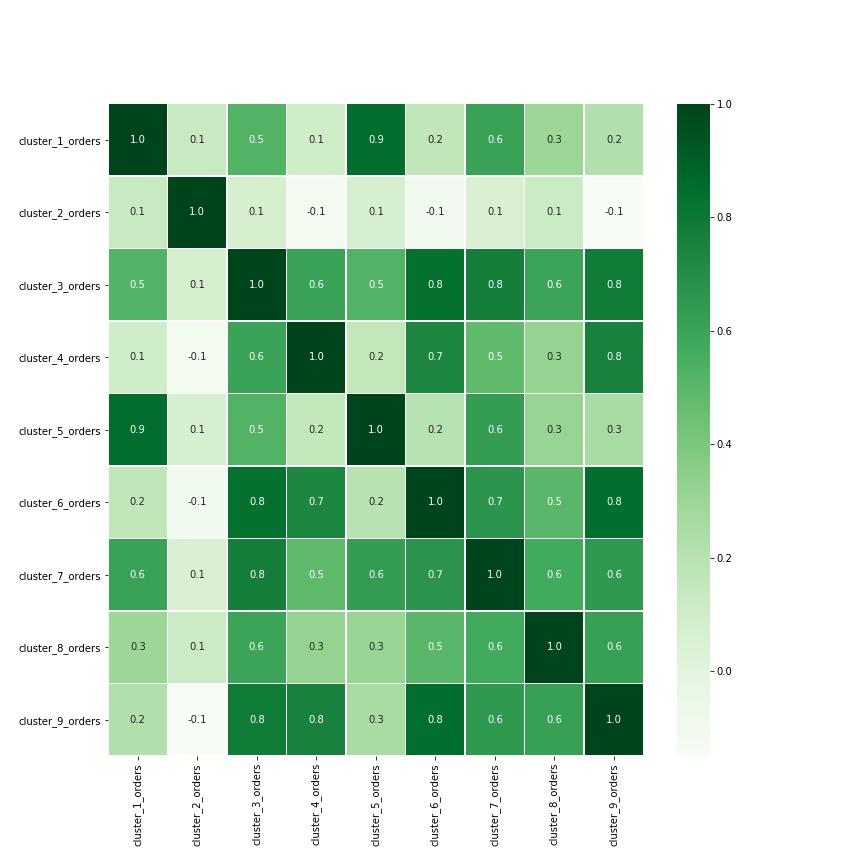
\includegraphics[width=\textwidth, height=0.6\textheight]{Images/cluster_corr_heatmap.jpg}
    \caption{Correlation heatmap for 9 clusters}
    \label{fig:Correlation heatmap for 9 clusters}
\end{figure}

\noindent We can observe from the sample correlation heatmap in Figure 16 that there exist strong correlation between certain clusters (like cluster 3 and 4 and cluster 6 and 8). To exploit the spatial correlation effects, each cluster is treated as a variable and VAR model was then trained on the clusters and used to predict the total demand for each of the clusters. 


\subsection{Assigning total cluster demand to individual location}

After we attained the total demand for each cluster, the next step would be to reallocate the total demand to each individual location in the cluster, making sure that the distribution of demand across the locations are relatively similar to as before. 

\noindent One assumption that was made here is that the distribution of the demand across the locations in each cluster remain relatively constant over time. Taking the previous distribution into account, the predicted demand for each cluster would then be reallocated to each individual location in the cluster using this equation:

\begin{center}
    $\displaystyle y_{i} = Y_{C(i)} * \frac{(\sum_{j=1}^{n}x_{ij})}{D_{C(i)}} \: \forall \: i$
\end{center}

\noindent where $y_i$ represents the predicted demand for location i, $Y_{C(i)}$ represents the predicted total demand of Cluster i, $C(i)$ represents the cluster which location i belongs to, $D_{C(i)}$ represents the total demand (from training set) of the cluster C(i).


\subsection{Results}

We also test the effect of different number of cluster groups on the MSFE on our full dataset. 

\begin{table}[H]
\begin{tabular}{|l|l|l|l|l|}
\hline
                                                                                                                          & \textbf{3 Clusters} & \textbf{6 Clusters} & \textbf{9 Clusters} & \textbf{12 Clusters} \\ \hline
\textbf{\begin{tabular}[c]{@{}l@{}}Clustering using euclidean\\ distance of latitude/longitude\end{tabular}}              & 61.18               & \textbf{60.67}      & 61.03               & 62.24                \\ \hline
\textbf{\begin{tabular}[c]{@{}l@{}}Clustering using correlation \\ between time series as distance\\ metric\end{tabular}} & 62.66               & 59.96               & \textbf{57.72}              & 61.60       \\ \hline
\textbf{\begin{tabular}[c]{@{}l@{}}Clustering using DTW as\\ distance metric\end{tabular}}                                & 64.00               & 64.37      & 62.68 & \textbf{62.20}                
\\ \hline
\end{tabular}
\caption{MSFE for different clustering distance metrics and number of clusters. Bolded results signifying the best result for the respective distance metric.}
\end{table}

\noindent Based on the results, the best model chosen would be clustering the data into 9 clusters using correlation between the time series as the distance metric.

\newpage
\section{Results and Conclusion}
The table below summarises the results of our models. 

\begin{table}[H]
\begin{tabular}{|l|l|l|ll}
\cline{1-3}
                                                                                                             & \textbf{\begin{tabular}[c]{@{}l@{}}MSFE (Locations with at \\ least 50 non-zero counts)\end{tabular}} & \textbf{MSFE (All locations)} &  &  \\ \cline{1-3}
\textbf{ARIMA}                                                                                               & 47.60                                                                                              & 72.48                         &  &  \\ \cline{1-3}
\textbf{GLM}                                                                                                 & 38.16                                                                                              & 82.42                         &  &  \\ \cline{1-3}
\textbf{VAR}                                                                                                 & 42.76                                                                                              & 76.72                         &  &  \\ \cline{1-3}
\textbf{VARX}                                                                                                & 41.73                                                                                              & 75.63                         &  &  \\ \cline{1-3}
\textbf{\begin{tabular}[c]{@{}l@{}}3-step approach (Using K-means \\ on geographical location)\end{tabular}} & 40.43 & 60.67                        &  &  \\ \cline{1-3}
\textbf{\begin{tabular}[c]{@{}l@{}}3-step approach (Using \\ K-means on correlation \\ of time series)\end{tabular}}           & 39.49 & \textbf{57.72}                         &  &  \\ \cline{1-3}
\textbf{\begin{tabular}[c]{@{}l@{}}3-step approach (Using \\ K-means on DTW \\ of time series)\end{tabular}}           & 40.10 & 62.20                         &  &  \\ \cline{1-3}
\end{tabular}
\caption{MSFE of the different methods used in this paper}
\end{table}


\noindent We can see that the VAR and VARX model performs better than the GLM models on the full dataset, suggesting that the spatial relationship between locations are useful in forecasting. Also, VARX performs better than VAR model in both cases, suggesting the exogenous variables have some explanatory power and do improve the forecast accuracy. 

\noindent Applying the 3-step forecast also gives a much improved result. This might be due to using a more reliable and reasonable model to predict total demands for just 9 clusters and then re-assigning it to individual locations, rather than having a model to predict all 839 locations, which would intuitively have higher error rate. The method of using VAR on all locations produced a relatively worse result, which is similar to the findings from \cite{Abolfazl2017}, which states that a simple VAR model would not perform as well for high-dimensional data.

\noindent As for the distance metric used for clustering, using correlation between the time series gives us the best result. This might be because correlation compares the general shape and trend of the time series regardless of scale, whereas for DTW, it is more effective to compare time series of varying length and speed. Using correlation also gives better results than using euclidean distance between the geo-locations, and this imply that spatial correlation is not limited to just geographical proximity but also on the time series similarity. 

\section{Limitations and Future Work}
Our 3-step approach model display decent MSFE result. However, using VAR is still technically a linear model and future work could include exploring using non-linear models like neural network, such as Long Short-Term Memory (LSTM) models or Convolutional LSTM models that also uses spatial-temporal features to forecast the demand across locations. LSTM or neural network models are also believed to be able to take into account the non-stationarity of the time series, which would allow our model to be more flexible without the need for differencing, which might lead to over-differencing for some series. 

\noindent Another area that could be explored further would be the method used to assign the total cluster demand to individual locations. Currently, the method simply used the historical distribution of the total sum of demand of each location over all the locations in that cluster. This would only work well if the distribution of the demand for the locations remain relatively constant over time. However, if the distribution of the locations fluctuates greatly, the current reassignment formula might not give a good result. Instead, we could try predict the distribution of the locations in each cluster or other methods to get a relatively stable and reasonable distribution over time.

\newpage
\section{Appendix}
\subsection{Distribution Plots of Exogenous Variables}
\begin{figure}[H]
    \centering
    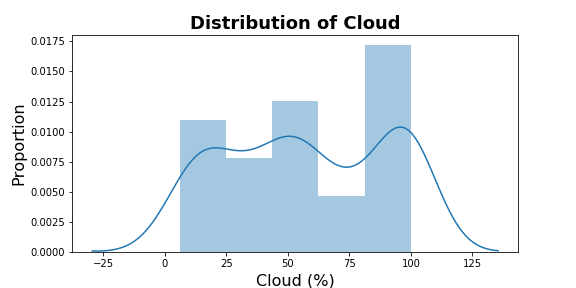
\includegraphics[width=0.6\textwidth, height=0.3\textheight]{Images/distplot_cloud.png}
    \caption{Distribution of Cloud}
    \label{fig:Distribution of Cloud}
\end{figure}

\begin{figure}[H]
    \centering
    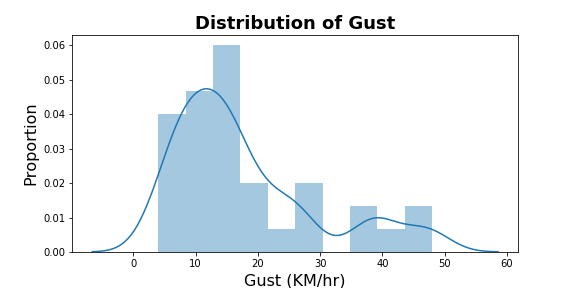
\includegraphics[width=0.6\textwidth, height=0.3\textheight]{Images/distplot_gust.png}
    \caption{Distribution of Gust}
    \label{fig:Distribution of Gust}
\end{figure}

\begin{figure}[H]
    \centering
    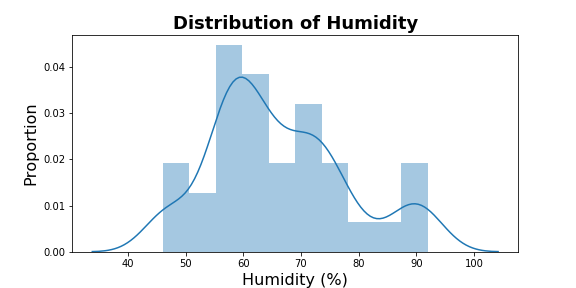
\includegraphics[width=0.6\textwidth, height=0.3\textheight]{Images/distplot_humidity.png}
    \caption{Distribution of Humidity}
    \label{fig:Distribution of Humidity}
\end{figure}

\begin{figure}[H]
    \centering
    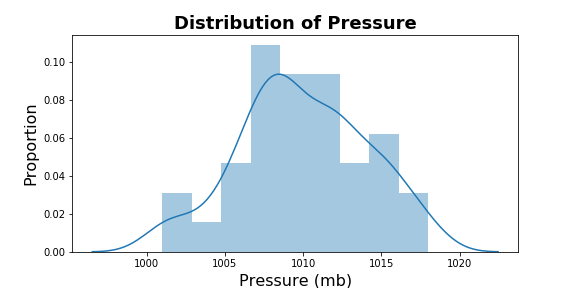
\includegraphics[width=0.6\textwidth, height=0.3\textheight]{Images/distplot_pressure.png}
    \caption{Distribution of Pressure}
    \label{fig:Distribution of Pressure}
\end{figure}

\begin{figure}[H]
    \centering
    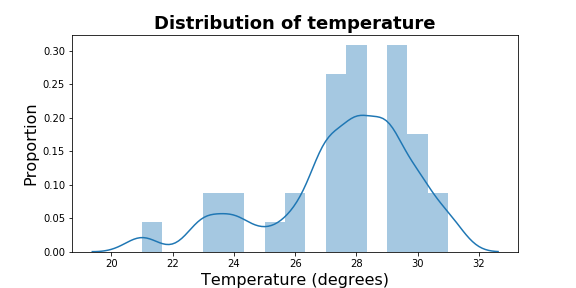
\includegraphics[width=0.6\textwidth, height=0.3\textheight]{Images/distplot_temp.png}
    \caption{Distribution of Temperature}
    \label{fig:Distribution of Temperature}
\end{figure}

\begin{figure}[H]
    \centering
    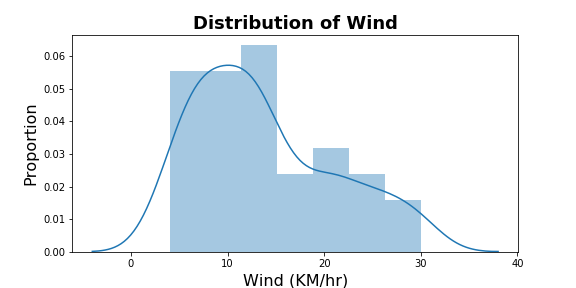
\includegraphics[width=0.6\textwidth, height=0.3\textheight]{Images/distplot_wind.png}
    \caption{Distribution of Wind}
    \label{fig:Distribution of Wind}
\end{figure}

\subsection{Mean Demand Against Exogenous Variables}

\begin{figure}[H]
    \centering
    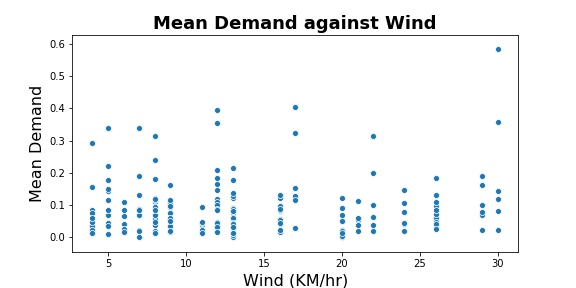
\includegraphics[width=0.6\textwidth, height=0.3\textheight]{Images/wind_mean_demand.jpg}
    \caption{Mean Demand against Wind}
    \label{fig:Mean Demand against Wind}
\end{figure}

\begin{figure}[H]
    \centering
    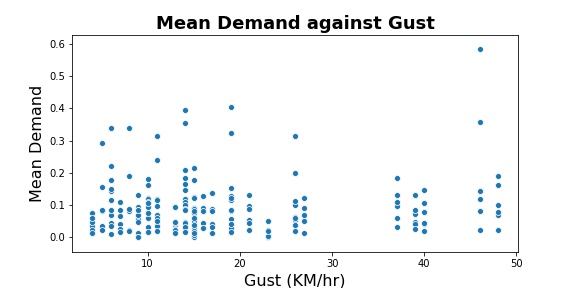
\includegraphics[width=0.6\textwidth, height=0.3\textheight]{Images/gust_mean_demand.jpg}
    \caption{Mean Demand against Gust}
    \label{fig:Mean Demand against Gust}
\end{figure}

\begin{figure}[H]
    \centering
    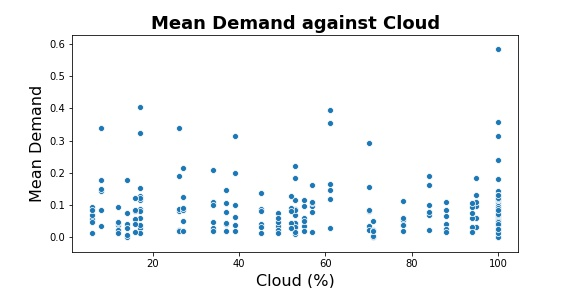
\includegraphics[width=0.6\textwidth, height=0.3\textheight]{Images/cloud_mean_demand.jpg}
    \caption{Mean Demand against Cloud}
    \label{fig:Mean Demand against Cloud}
\end{figure}

\begin{figure}[H]
    \centering
    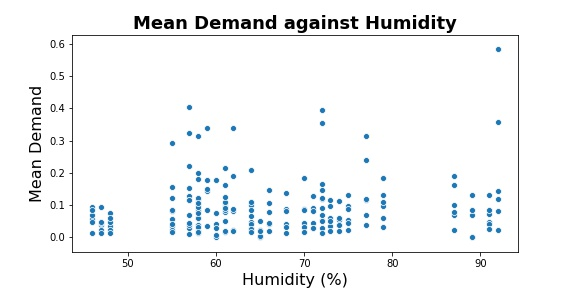
\includegraphics[width=0.6\textwidth, height=0.3\textheight]{Images/humidity_mean_demand.jpg}
    \caption{Mean Demand against Humidity}
    \label{fig:Mean Demand against Humidity}
\end{figure}

\begin{figure}[H]
    \centering
    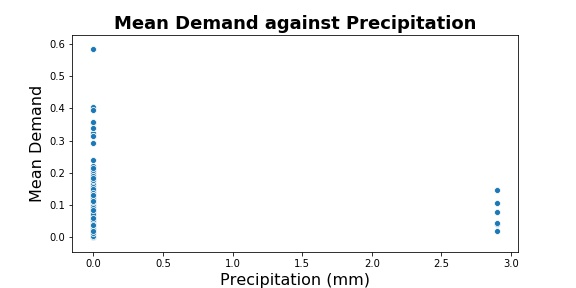
\includegraphics[width=0.6\textwidth, height=0.3\textheight]{Images/prec_mean_demand.jpg}
    \caption{Mean Demand against Precipitation}
    \label{fig:Mean Demand against Precipitation}
\end{figure}
\newpage
%%%%%%%%%%%%%%%%%%%%%%%%%%%%%%%%%%%%%%%%%%%%%%%%%%%%%%%%%%%%
%%% Bibliography
%%%%%%%%%%%%%%%%%%%%%%%%%%%%%%%%%%%%%%%%%%%%%%%%%%%%%%%%%%%%
\bibliographystyle{abbrv} 
\bibliography{references}


\end{document}
